% for sharelatex https://www.sharelatex.com/github/
% !TEX program = pdflatex

\documentclass[hyper]{tufte-handout}
\usepackage{morefloats}

% \providecommand{\url}[1]{\texttt{#1}}
% \providecommand{\urlprefix}{URL }
% \expandafter\ifx\csname urlstyle\endcsname\relax
%   \providecommand{\doi}[1]{doi:\discretionary{}{}{}#1}\else
%   \providecommand{\doi}{doi:\discretionary{}{}{}\begingroup
%   \urlstyle{rm}\Url}\fi
% \providecommand{\bibAnnoteFile}[1]{%
%   \IfFileExists{#1}{\begin{quotation}\noindent\textsc{Key:} #1\\
%   \textsc{Annotation:}\ \input{#1}\end{quotation}}{}}
% \providecommand{\bibAnnote}[2]{%
%   \begin{quotation}\noindent\textsc{Key:} #1\\
%   \textsc{Annotation:}\ #2\end{quotation}}
% \providecommand{\eprint}[2][]{\url{#2}}


% Set up the images/graphics package
\usepackage{graphicx}
\setkeys{Gin}{width=\linewidth,totalheight=\textheight,keepaspectratio}
\graphicspath{{figures/}}

% The following package makes prettier tables.  We're all about the bling!
%\usepackage{booktabs}

% The units package provides nice, non-stacked fractions and better spacing
% for units.
% \usepackage{units}

% The fancyvrb package lets us customize the formatting of verbatim
% environments.  We use a slightly smaller font.
% \usepackage{fancyvrb}
% \fvset{fontsize=\normalsize}

% Small sections of multiple columns
% \usepackage{multicol}


\hypersetup{colorlinks}

% https://en.wikibooks.org/wiki/LaTeX/Hyperlinks#.5Chyperref
% http://www.tug.org/applications/hyperref/manual.html#x1-120003.8
% \hypersetup{
%     pdfauthor={},
%     pdftitle={Tufte-LaTeX document},
%     pdfsubject={subject},
%     pdfkeywords={}
% }
% \href{http://example.com}{test}
% \href{http://www.wikibooks.org}{Wikibooks home}
% http://tex.stackexchange.com/questions/66526/what-is-the-right-way-to-use-hyperref-options-with-tufte-handout-class

\newcommand{\etal}{\textit{et. al.}}
%\newcommand{\scite}[3]{\sidenote{#1 \etal\ #2, \url{#3}}}
%\newcommand{\scite}[3]{(#1 \etal\ #2)\sidenote{\url{#3}}}
\newcommand{\scite}[3]{\sidenote{\href{#3}{#1 \etal\ #2.}}}
\newcommand{\scitetwo}[3]{\sidenote{\href{#3}{#1 #2.}}}

\title{Research Statement}
\author{\href{http://matsen.fredhutch.org/}{Frederick Matsen}, Fred Hutchinson Cancer Research Center}


\begin{document}

\maketitle

\begin{abstract}
\noindent
My work at the Fred Hutch has been to develop and apply methods at the intersection of biomedicine and evolutionary molecular sequence analysis.
I have especially focused on methods that that incorporate uncertainty using a likelihood-based framework and leverage hidden evolutionary structure of the data.
\end{abstract}


\newthought{Model-based statistical inference provides a unified framework} to learn from plentiful, indirect, and often noisy biological data.\sidenote{%
Here \textit{model-based} means that our ideas about how the system works are formalized into a probabilistic model.
\textit{Statistical inference} means that uncertainty in measurement is pushed all the way through to obtain parameter estimates with appropriate statements of confidence in those estimates.}
Biological data also often comes with hidden evolutionary structure, such as that formed by a phylogenetic (i.e.\ evolutionary) tree that can be productively incorporated into an analysis.
Biology furnishes a never-ending supply of inferential challenges in this area; I will narrate our application of these principles through our collaborative work.


\section{Evolution of viruses and the immune system}
We have enjoyed working on a number of questions concerning viral diversity and evolution as driven by host innate and adaptive immune systems.
The random nature of this process, as well as a very large population of viruses from which we sample only a small fraction, serves to illustrate useful features of model-based inference.
One question of central importance to Dr. Julie Overbaugh's HIV research concerns \textit{superinfection}: infection with a distinct lineage of a virus through a separate infection event.
Given a sample of viral molecular sequences, or a series of such samples, one would like to understand the level of evidence for a superinfection event.
Assuming a reasonable amount of difference between the original and superinfecting lineages, one can phrase the superinfection hypothesis in phylogenetic terms:
to what extent do we think that those viral molecular sequences came from two distinct lineages?
With a model-based analysis we can incorporate (somewhat) complex mutational processes into a
\textit{likelihood function}\sidenote{The likelihood function of a parameter set can be thought of as giving the likelihood of generating the observed data with those model parameters.}
that evaluates how well a collection of model parameters fits the data.
This is in contrast to non-model approaches such as maximum parsimony, for which the objective is set \textit{a priori} without modeling the molecular evolution process.
There is considerable uncertainty in HIV phylogeny given a sample of molecular sequences, due both to HIV's fast evolutionary rate and due to the inadequacy of our models for its molecular evolution.
For this reason we \emph{integrate out the uncertainty in this evolutionary reconstruction} in order to quantify the support for a superinfection hypothesis.\scite{Ronen}{2013}{http://dx.doi.org/10.1371/journal.ppat.1003593}

We have taken such a likelihood-based approach to problems in viral evolution and diversity
to investigate the evolutionary impact of pre-exposure HIV prophylaxis,\scite{Lehman}{2015}{http://dx.doi.org/10.1093/infdis/jiu677}
to study simian foamy virus in its natural\scite{Lee}{2013}{http://dx.doi.org/10.1038/emi.2013.23}
and human\scite{Engel}{2013}{http://dx.doi.org/10.1038/emi.2013.60} host,
as well as to study the zoonotic transfer of Astrovirus.\sidenote{In press.}
We have also investigated how the innate immune system impacts viral evolution, including the
evolution of anti-restriction factor genes in viruses,\scite{Lim}{2012}{http://dx.doi.org/10.1016/j.chom.2012.01.004}
how such dynamics shaped the ancestor of HIV-1,\scite{Etienne}{2013}{http://dx.doi.org/10.1016/j.chom.2013.06.002}
and how viral restriction by APOBEC3G may be the reason why simian foamy virus does not replicate extensively in the human host.\scite{Matsen}{2014}{http://dx.doi.org/10.1371/journal.pcbi.1003493}

\begin{marginfigure}%
  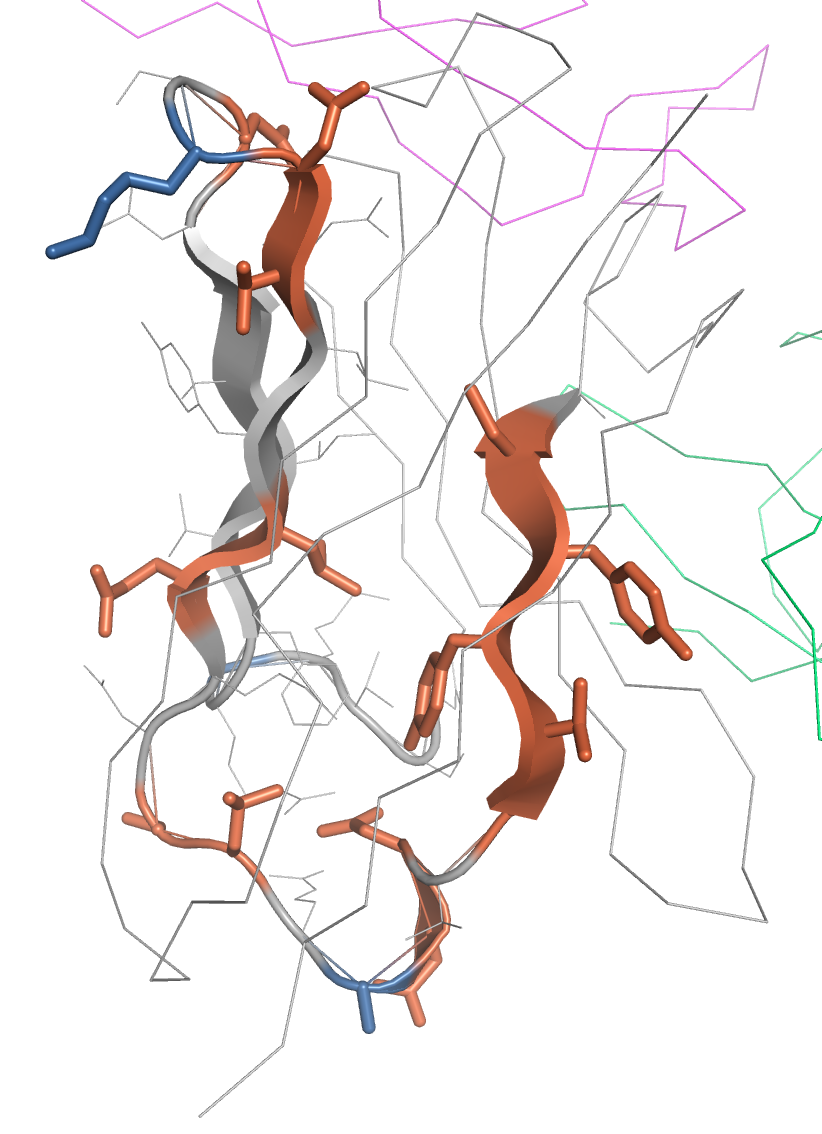
\includegraphics[width=1.5in]{bcell-structure.png}
  \caption{\
    Protein structure of a sequenced portion of the heavy chain colored by selection inference.
    Purifying selection marked orange and diversifying selection marked blue.
    }
  \label{FIGbcell}
\end{marginfigure}

We have recently become very interested in how the \textit{adaptive} immune system continually evolves within each individual in order to neutralize and destroy pathogens.
Specifically, we have embarked on a program to bring modern model-based statistical inference to the within-host evolution of antibody-making B cells.
Although the elements of B cell affinity maturation are the same as molecular evolution in other settings, being based on recombination, point mutation, and selection, there are a number of important differences.
Postdoc Duncan Ralph and I have developed means to infer the un-mutated ancestors of B cell receptor sequences using detailed hidden Markov models (HMMs), resulting in significantly better results than previous methods \scite{Ralph}{2015}{http://arxiv.org/abs/1503.04224}.
We then used this framework to develop the first likelihood-based approach to infer ``clonal families,'' which are collections of B cells that descend from the same common ancestor \sidnote{Submitted.}
We have developed new methods to do evolutionary selection inference in the setting of many reads of varying length\scite{McCoy}{2015}{http://dx.doi.org/10.1098/rstb.2014.0244} and have applied them to the inference of selection happening on B cell receptor V gene (Figure~\ref{FIGbcell}).
We are approaching the very strong context dependence of mutation by comparing per-site models to composite likelihood strategies in order to better reconstruct the history of mutation events leading to observed B cell receptor sequences (joint with Peter Ralph, USC).

\section{Using geometry to better integrate over phylogenetic trees}
\begin{marginfigure}%
  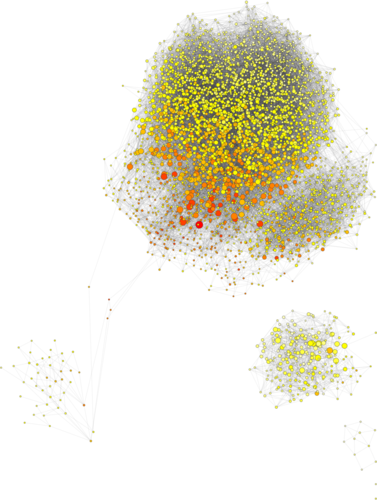
\includegraphics[width=1.5in]{ds6_small.png}
  \caption{\
    The top 4096 trees found by an inference procedure.
    Vertices represent trees, and edges represent subtree-prune-regraft (SPR) moves (Figure~\ref{FIGsprdef}).
    Disconnected sets show peaks in the likelihood surface.
    }
  \label{FIGsprmix}
\end{marginfigure}
All model-based phylogenetic inference methods start with a heuristically constructed tree and then proceed through a series of random modifications of the tree whereby modifications that result in better (higher likelihood) trees are favored over jumps to lower likelihood trees.
Although there are certain guarantees concerning how phylogenetic reconstruction methods will perform if run for an infinite period of time, rather little is known about how these methods work when run in the real world on real data.
For example, there may be two ``peaks'' of good phylogenetic trees separated by a ``trough''; it may take an arbitrarily long time to cross between the peaks with high probability (Figure~\ref{FIGsprmix}).
Such behavior will manifest itself in overconfidence in the tree represented by the first peak selected.

\begin{marginfigure}%
  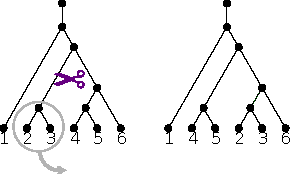
\includegraphics[width=1.85in]{spr-definition.pdf}
  \caption{\
    A phylogenetic tree and the result of applying a subtree-prune-regraft (SPR) modification to it.
    In this modification, a subtree is cut off the larger tree, then reattached using a new edge (dotted line of right hand tree).
    }
  \label{FIGsprdef}
\end{marginfigure}
Thus, in order to make confident statements it is necessary to gain an understanding of how these likelihood surfaces look on real data.
Postdoc Chris Whidden and I have explored these surfaces by equipping the collection of trees with a geometry corresponding to \textit{subtree-prune-regraft (SPR)} moves (Figure~\ref{FIGsprdef}).
In this tree modification, part of a tree is detached and then re-attached at another location.
These SPR moves are the canonical example of the type of tree modification done in phylogenetic inference as described above.

Our work enables analysis of the proximate causes of bad behavior of phylogenetic inference procedures by finding peaks and troughs in a graph representation of the set of phylogenetic trees.\scite{Whidden}{2015}{http://dx.doi.org/10.1093/sysbio/syv006}
We have also made some progress to understanding the ultimate causes of difficulty of movement in the SPR graph by quantifying large-scale features of the graph via the Ricci-Ollivier curvature \scite{Whidden}{2015}{http://arxiv.org/abs/1504.00304}.
In the process we have characterized the symmetries of this graph induced by relabeling pairs of trees\scite{Matsen}{2015}{http://arxiv.org/abs/1507.04784}\scite{Billey}{2015}{http://arxiv.org/abs/1507.04976}.
We are also exploring the degree to which conflicting signals in sequence alignments may contribute to such problems.

This work has also made us quite curious about the shape of the phylogenetic likelihood function.
Postdoc Vu Dinh and I performed a careful examination of the phylogenetic likelihood function as a function of a single branch length, finding that it is guaranteed to have a single maximum for simple models but may have an arbitrary number of maxima for more complex models and pathological data\scite{Dinh}{2015}{http://arxiv.org/abs/1507.03647}.
We have built a corresponding surrogate function for one-dimensional phylogenetic likelihood functions that can be used to quickly sample from an approximate posterior\sidenote{In preparation.}.

\section{Incorporating phylogenetic structure into ecological analysis}
\begin{marginfigure}%
  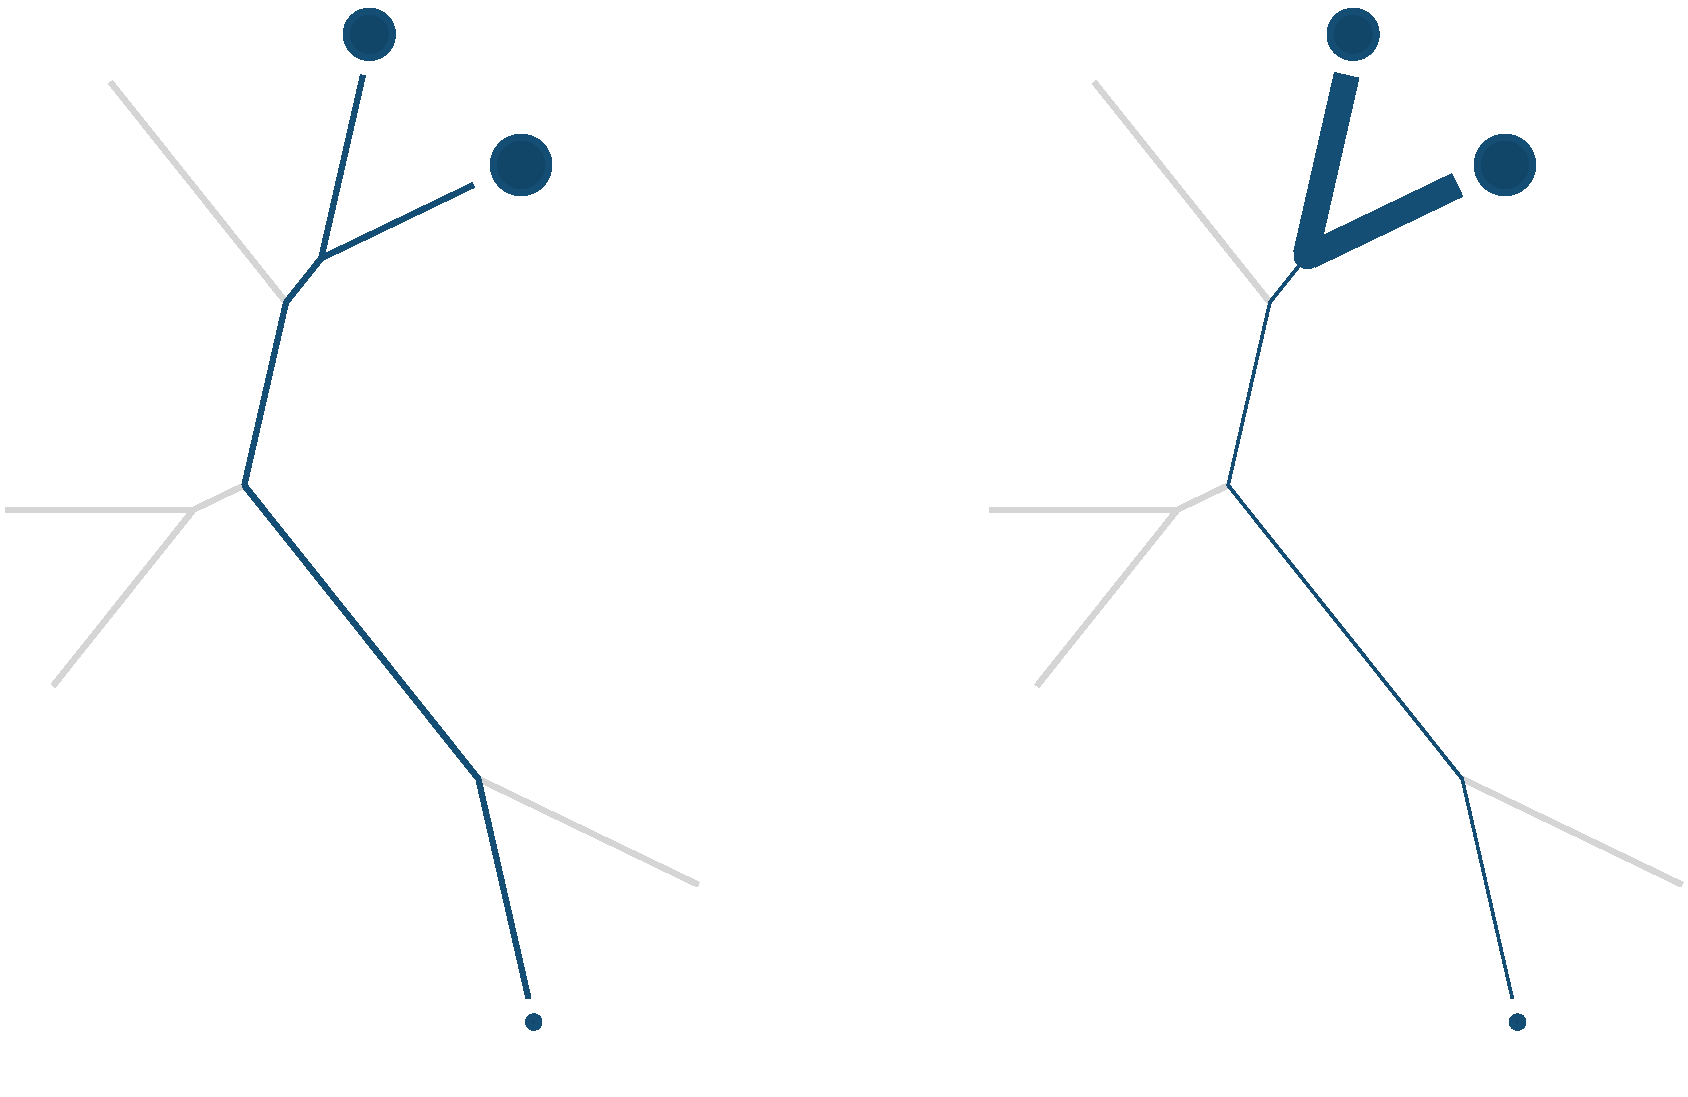
\includegraphics[width=2in]{pd.pdf}
  \caption{\
    Cartoon of unweighted phylogenetic diversity (left) and an abundance-weighted phylogenetic diversity measure (right), where taxa present in a sample are shown as circles and abundances are shown as the size of the circles.
    }
  \label{FIGpd}
\end{marginfigure}

Evolution also endows ecological data with added structure, which we may want to incorporate into a comparative analysis.
For example, if a pair of communities harbors similar organisms between them, we might want to call those communities more similar than if a pair of communities harbors very different organisms.
I have worked a considerable amount to bring such structure into statistical analysis of ecological data, motivated by human microbiome research happening at the Fred Hutch.

This work can be classified into two categories: within-sample diversity analysis and between-sample comparison.
For within-sample diversity, the canonical formulation in a phylogenetic context is called \textit{phylogenetic diversity}, and is defined as the total amount of branch length (evolutionary distance) between all species in a sample.
I have extended this work in two directions.
First, I derived closed-form equations for the expectation and variance of phylogenetic diversity under sub-sampling, which can help quantify a ``confidence interval'' on diversity estimates.\scitetwo{Nipperess and Matsen}{2013}{http://dx.doi.org/10.1111/2041-210X.12042}
Second, I found with my programmer Connor McCoy, that partially abundance-weighted phylogenetic diversity estimates were most informative in distinguishing between normal and dysbiotic states.\scitetwo{McCoy and Matsen}{2013}{http://dx.doi.org/10.7717/peerj.157}

Estimates of the differences between samples also benefit from incorporation of phylogenetic structure.
In fact, microbial ecology researchers had already been making use of such phylogenetic structures in sample comparison for many years before Steve Evans and I found that their comparison framework was a special case of a comparative framework developed in the late 18th century.\scitetwo{Evans and Matsen}{2012}{http://dx.doi.org/10.1111/j.1467-9868.2011.01018.x}
We also were able to integrate phylogenetic structure into ordination and clustering analysis directly,\scitetwo{Matsen and Evans}{2013}{http://dx.doi.org/10.1371/journal.pone.0056859} rather than first reduce samples to a sample-by-sample pairwise distance matrix.
We are currently extending this work to incorporate both discrete and continuous aspects of the phylogenetic tree into a similar framework.\sidenote{In preparation.}

In addition, I have developed methods for finding an appropriate set of molecular sequences to use as a ``reference database'' for comparative analysis.
This includes adapting a ``coloring'' problem previously described in the computer science literature to describe the discord between a phylogenetic tree on a collection of sequences and their taxonomic annotation,\scitetwo{Matsen and Gallagher}{2012}{http://dx.doi.org/10.1186/1748-7188-7-8} with the goal of finding troublesome aspects of the phylogenetic tree or the taxonomy.
We also developed the first exact algorithm for selecting a set of representatives in a phylogenetic tree that minimize the average distance to the closest leaf for a collection of sequence reads.\scite{Matsen}{2013}{http://dx.doi.org/10.1093/sysbio/syt044}
We use both of these results in our pipeline to develop automated customized reference databases for human body sites\sidenote{In preparation.} to reduce the need for expert curation of specialized sequence databases.


\section{Professional service}

In additional to the usual academic professional service, I have started and continue to lead three initiatives to improve the research landscape in my field and at the Fred Hutch.
Since 2009 I have run \url{http://phyloseminar.org/}, an online lecture series which has had 50 talks on a wide variety of phylogenetic inference and applications.
The seminar video recordings are on YouTube, and have been watched for over 950 hours within the last year.
In 2014 year I started a sister project, \url{http://phylobabble.org/}, an electronic forum to discuss best practice and new developments in phylogenetics.
In 2014 I also started \url{http://fredhutch.io/}, an initiative to facilitate education about and promote access to computational resources at the Fred Hutch.
We have built out a full-featured \href{http://usegalaxy.org/}{Galaxy} instance used extensively by Fred Hutch researchers with no programming experience to analyze their data.
We are also offering 7 week introductory bioinformatics courses to the Fred Hutch community and have made course materials \href{http://fredhutchio.github.io/intro-bioinformatics/}{available online}.
These courses have been wildly popular, with a waiting list many times longer than course capacity.

% \bibliography{research}
% \bibliographystyle{unsrt}

\end{document}

